\chapter{FUNDAMENTAÇÃO TEÓRICA}

Neste capítulo encontram-se os conceitos e fundamentos teóricos das tecnologias que foram utilizadas nesta dissertação, como o \emph{Ethernet Energy Efficient}, \emph{Packet Coalescing}, \emph{Random Early Detection}, \emph{Controlled Delay}, \emph{Explicit Congestion Notification}, \emph{MapReduce} e Hadoop. Além disso, é exposta a necessidade de estudos adicionais devido à constante evolução da área e ferramentas contidas nela.

\section{Energy Efficient Ethernet}

O \emph{Energy Efficient Ethernet} também conhecido como IEEE802.3az, ou ainda \emph{Green Ethernet}, é um protocolo de rede aprovado em 2010 pelo Instituto de Engenheiros Eletricistas e Eletrônicos (\emph{Institute of Electrical and Electronics Engineers} - IEEE). Como a Ethernet é a tecnologia dominante para LANs com fio, espera-se que os mecanismos de economia de energia do EEE tragam economias de energia consideráveis \cite{de2013performance}. O EEE já foi implantado, mas, os fornecedores de sistemas e máquinas aconselham seus clientes a desabilitá-lo em seu uso diário \cite{DellEEE}; \cite{ethernet2011ieee}, uma vez que seu impacto é mal compreendido em aplicações reais, não deixando claro o benefício em relação à economia de energia e desempenho.

\subsection{Deep Sleep Mode}

O EEE802.3az no modo \emph{Deep Sleep} funciona da seguinte maneira: Quando uma estação transmissora de um \emph{link} com esse protocolo detecta uma baixa utilização do \emph{link}, ela pode solicitar que o transmissor PHY local entre no modo \emph{Low Power Idle} (LPI) e envie símbolos apropriados pelo \emph{link}. Ao receber e decodificar esses símbolos, o receptor do parceiro de \emph{link} pode entrar no modo LPI, gerando assim economia de energia. Os caminhos de transmissão e recepção podem entrar e sair dos estados de baixa energia de forma independente. A energia é conservada desativando os blocos funcionais correspondentes do caminho individual \cite{5621025}.

\begin{figure}[htp]
    \centering
    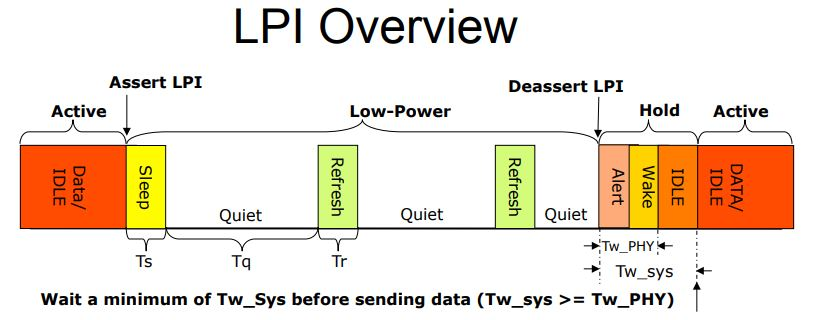
\includegraphics[width=16cm]{2-fundam/Figura_1.jpg}
    \caption{Overview of EEE LPI Operation}
    \cite{EEEOverview}
    \label{fig:eeelpi}
\end{figure}

Quando o início da codificação `\emph{Assert LPI}' no xMII (\emph{Media Independent Interface}) é detectado, os sinais PHY (camada física que provê uma interface entre a subcamada MAC e o canal do rádio) hibernam para seu parceiro de \emph{link}, para indicar que o transmissor local está entrando no modo LPI como observamos na figura 2.1.

A capacidade EEE na maioria dos PHYs (por exemplo, 100BASE-TX, 10GBASE-T, 1000BASE-KX, 10GBASEKR e 10GBASE-KX4) requer que o transmissor PHY local fique no modo \emph{Quiet} após o modo \emph{Low-Power} ser sinalizado.  No modo 1000BASE-T LPI, o transmissor PHY local fica \emph{Quiet} somente depois que o PHY local sinaliza para o modo \emph{Sleep} e recebe um sinal de \emph{Sleep} do PHY remoto. Se o PHY remoto optar por não sinalizar o modo LPI, nenhum dos PHY pode entrar no modo de baixa energia; no entanto, as solicitações LPI são passadas de uma extremidade do \emph{link} para a outra independentemente, e a economia de energia do sistema pode ser alcançada mesmo se o \emph{link} PHY não entrar em um modo de baixa energia \cite{5621025}.

A função de transmissão do PHY local é habilitada periodicamente para transmitir sinais de atualização que são usados pelo parceiro de \emph{link} para atualizar filtros adaptativos e circuitos de temporização a fim de manter a integridade do \emph{link}. Este ciclo de atualização silenciosa continua até a recepção da codificação normal entre quadros no xMII. A função de transmissão no PHY comunica isso ao parceiro de \emph{link}, enviando um sinal de despertar por um período de tempo predefinido. O PHY então entra no estado operacional normal novamente.

De acordo com \cite{reviriego2010burst}, a eficiência de energia do EEE é impactada por dois fatores: o consumo de energia ocioso - cerca de 10\%; e as despesas gerais de \emph{Wake}/\emph{Sleep}. O consumo de energia ocioso possuí um custo fixo, que não é afetado pela entrada ou saída do modo LPI, e reflete apenas nas despesas gerais de \emph{Wake}/\emph{Sleep}. Quando a carga é moderada à alta, a sobrecarga de energia da transição para dentro e fora do modo LPI podem ser amortizadas em vários pacotes. Entretanto, quando a carga é moderada à baixa, pode ser necessário despertar e hibernar o \emph{link} de conexão para transmitir um único \emph{frame}, resultando em penalidades de gastos altos de energia e latência em termos relativos.

\begin{table}[!htp]
\centering
\caption{EEE 150-byte frame Efficiency}
\label{tabela150byte}
\begin{tabular}{|c|cccc|}
\cline{2-5}
\multicolumn{1}{c|}{}& Min. \emph{Tw} (µs) &  Min. \emph{Ts} (µs) &  Min. \emph{Tframe} (µs) & Efficiency (\%) \\
\hline
\texttt{100Base-TX} & 30,5 & 200 & 12 & 4,9 \\
\hline
\texttt{1000Base-T} & 16,5 & 182 & 1,2 & 0,6 \\
\hline
\texttt{10GBase-T} & 4,48 & 2,88 & 0,12 & 1,6 \\
\hline
\end{tabular}
\end{table}

Pode-se observar na tabela 2.1, em alguns momentos é necessário sair do Modo LPI para transmitir um único ou poucos \emph{frames}, o que resulta em um acumulo de latência na rede como mencionado em \cite{reviriego2010burst}, além da perda de eficiência, que em alguns casos pode chegar a apenas 0,6\% comparado a conexões comuns \emph{Ethernet}.

\begin{table}[!htp]
\centering
\caption{EEE 1500-byte frame Efficiency}
\label{tabela1500byte}
\begin{tabular}{|c|cccc|}
\cline{2-5}
\multicolumn{1}{c|}{}& Min. \emph{Tw} (µs) &  Min. \emph{Ts} (µs) &  Min. \emph{Tframe} (µs) & Efficiency (\%) \\
\hline
\texttt{100Base-TX} & 30,5 & 200 & 120 & 34,2 \\
\hline
\texttt{1000Base-T} & 16,5 & 182 & 12 & 5,7 \\
\hline
\texttt{10GBase-T} & 4,48 & 2,88 & 1,2 & 14 \\
\hline
\end{tabular}
\end{table}

Como esperado, os índices de alta economia de energia com EEE são atingidos quando os pacotes que devem ser transmitidos são maiores e em grande quantidade como demonstrado na tabela 2.2, em que podemos atingir até 34,2\% de eficiência energética em relação ao padrão \emph{Ethernet} comum.

Felizmente, o problema descrito na tabela 2.1 pode ser corrigido adicionando \emph{Active Queue Management} a rede, como demonstra o estudo do impacto da utilização de EEE com \emph{Packet Coalescing} e \emph{Active Queue Management} no Hadoop 1.x \cite{silva2018eon}. Entretanto, se faz necessário estudos destas mesmas configurações na linha do Hadoop 3.x que executa o \emph{MapReduce} através do YARN diferentemente da versão 1.x, e utiliza \emph{Erasure Coding} em seu armazenamento diferentemente das versões 1.x e 2.x. Estas informações estão detalhadas de uma forma abrangente no subtópico do Apache Hadoop neste mesmo capítulo.

\subsection{Fast Wake Mode}

\emph{Fast wake} refere-se ao modo pelo qual o transmissor continua a transmitir sinais durante o estado LPI para que o receptor possa retomar a operação com um tempo \emph{wake} mais curto (como exposto na figura 2.2). Para o processo de transmissão, além das codificações do LPI, não há diferença entre o \emph{Deep Sleep Mode} e o \emph{Fast Wake Mode} \cite{6891095}. O suporte ao modo \emph{Fast Wake} é obrigatório para PHYs com velocidade operacional de 40 Gb/s ou superior que implementam o EEE. Utilizar este modo resulta em um consumo energia do link em cerca de 60\% \cite{georgakoudis2019evaluating}; \cite{6891095}, um valor elevado se comparado aos 10\% do modo \emph{Deep Sleep}.

\begin{figure}[htp]
    \centering
    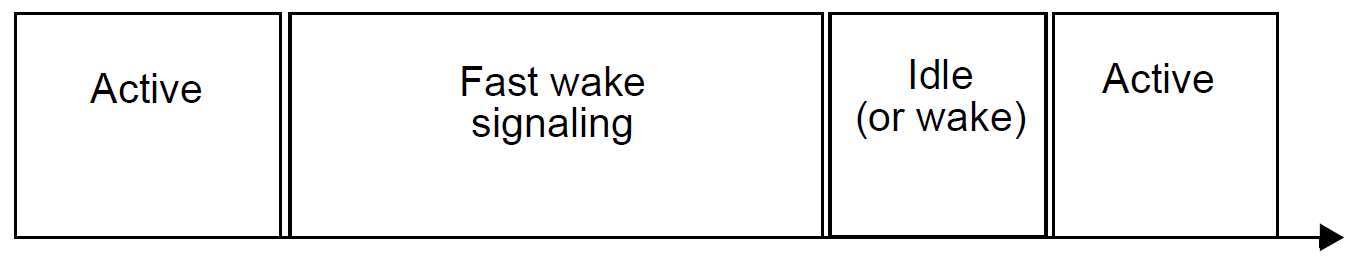
\includegraphics[width=11cm]{2-fundam/FastWakeMode.PNG}
    \caption{Overview of EEE fast wake operation}
    \cite{6891095}
    \label{fig:eeefastwakemode}
\end{figure}

\section{Packet Coalescing}

De uma forma simples, o \emph{Packet Coalescing} é o agrupamento de pacotes como forma de limitar o número de interrupções de recebimento e, como resultado, diminuir a quantidade de processamento necessária. Isso pode aumentar a latência da rede, mas em contrapartida, aumenta as chances de que a rede consuma menos energia, principalmente quando aliada ao EEE.

O \emph{Packet Coalescing}, do português Coalescência de Pacotes, é um método que inclui o recebimento de múltiplos pacotes de IP (\emph{Internet Protocol}). Cada um destes múltiplos pacotes de IP possuí um cabeçalho, além de um segmento de TCP (\emph{Transmission Control Protocol}) com cabeçalho, e um \emph{payload}, em que vários pacotes pertencentes a um mesmo fluxo TCP/IP são transmitidos. O método também inclui a preparação de um pacote de IP com um único cabeçalho de IP e um único segmento de TCP com um único cabeçalho de TCP e uma única carga formada por uma combinação das cargas de segmento de TCP dos vários pacotes de IP. O método inclui ainda a geração de um sinal que causa o processamento de recepção do pacote de IP \cite{makineni2020packet}.

Um estudo feito por \cite{mostowfi2011saving} estima que uma economia de energia potencial de 3,5 TWh/ano pode ser obtida pela implantação do \emph{Packet Coalescing} em todos os futuros \emph{switches} domésticos ou de pequenas empresas nos Estados Unidos. Outro artigo publicado por \cite{e2017energy} mostra que quando utilizado em redes de 10GbE nos \emph{clusters} \emph{MapReduce}, o \emph{Packet Coalescing} juntamente ao EEE proporciona uma economia de energética de 20\% a 60\%.

\begin{figure}[htp]
    \centering
    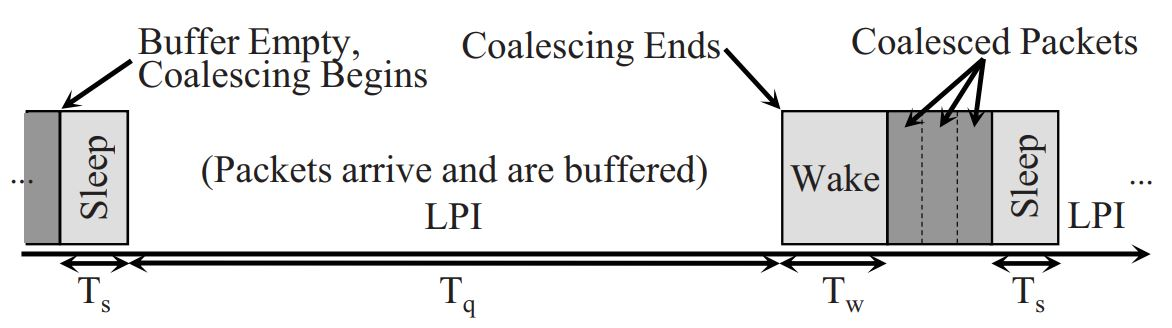
\includegraphics[width=11cm]{2-fundam/Figura_2.jpg}
    \caption{EEE with Packet Coalescing}
    \cite{mostowfi2011saving}
    \label{fig:EEEWithPacketCoalescing}
\end{figure}

Pode-se observar na figura 2.3 o resultado da junção do \emph{Packet Coalescing} com EEE. Conforme mostrado nesta figura, quando todos os pacotes na fila de transmissão (ou \emph{buffer}) são transmitidos e o \emph{buffer} fica vazio, o link é colocado no modo LPI com uma transição para o modo \emph{Sleep} que leva um tempo T\textit{s}. Os pacotes que chegam depois não são transmitidos imediatamente, mas são armazenados dentro de um \emph{buffer} de coalescência. Quando um tempo máximo passa da chegada do primeiro pacote ao \emph{buffer} de coalescência, ou o número de pacotes armazenados no \emph{buffer} atinge um número máximo predefinido, o link sai do modo LPI, o que leva um tempo T\textit{w}, e então, todos os pacotes coalescidos são transmitidos em uma única rajada \cite{mostowfi2011saving}.

\section{Active Queue Management}

\emph{Active Queue Management} é uma política implementada em roteadores e \emph{switches} para descartar pacotes dentro de um \emph{buffer} associado a um \emph{Network Interface Controller} (NIC) antes que o \emph{buffer} fique cheio, geralmente com o objetivo de reduzir o congestionamento da rede ou melhorar a latência de ponta a ponta \cite{adams2012active}. Esta tarefa é realizada pelo escalonador da rede, que para isso pode utilizar vários algoritmos como o \emph{Random Early Detection} (RED) \cite{floyd1993random} ou \emph{Controlled Delay} (CoDel) \cite{nichols2012controlling}.

Devido à simplicidade do mecanismo de enfileiramento \emph{First In First Out} (FIFO), as filas \emph{drop-tail} que descartam os pacotes de entrada quando a fila está cheia são as mais amplamente utilizadas na Internet atualmente. Infelizmente, quando confrontado com congestionamento persistente, as filas \emph{drop-tail} se enchem, resultando em atrasos maiores. Além disso, as filas \emph{drop-tail} também podem descartar vários pacotes, agravando a instabilidade do sistema e a imparcialidade da largura de banda. O \emph{Active Queue Management} (AQM) se propõe a substituir o gerenciamento de fila \emph{drop-tail} para melhorar o desempenho da rede em termos de atraso, utilização do \emph{link}, taxa de perda de pacotes e integridade do sistema. O AQM aprimora os roteadores para detectar e notificar os sistemas finais de congestionamento iminente com antecedência, permitindo que as fontes de tráfego reduzam suas taxas de transmissão antes que as filas de roteadores e comutadores congestionadas estourem \cite{chung2003analysis}.

\subsection{Random Early Detection}

Podemos observar o esquema do \emph{Random Early Detection} (RED) na figura 2.4. Este é um conhecido AQM leve que usa o tamanho médio da fila e o limite mínimo ({$\mathit{min}_\mathit{th}$}) e o limite máximo ({$\mathit{max}_\mathit{th}$}) para detectar o congestionamento iminente e determinar a probabilidade de notificação de congestionamento. Quando o tamanho médio da fila está entre ({$\mathit{min}_\mathit{th}$}) e ({$\mathit{max}_\mathit{th}$}), o RED descarta aleatoriamente (ou marca no modo ECN) os pacotes de entrada com uma probabilidade que aumenta linearmente de zero para a probabilidade máxima ({$\mathit{max}_\mathit{p}$}) conforme o tamanho médio da fila aumenta de ({$\mathit{min}_\mathit{th}$}) a ({$\mathit{max}_\mathit{th}$}). No entanto, quando o tamanho médio da fila é maior que ({$\mathit{max}_\mathit{th}$}), o RED descarta todos os pacotes de entrada até que o tamanho médio da fila caia abaixo de ({$\mathit{max}_\mathit{th}$}) \cite{floyd1993random}; \cite{lochin2011managing}.

\begin{figure}[htp]
    \centering
    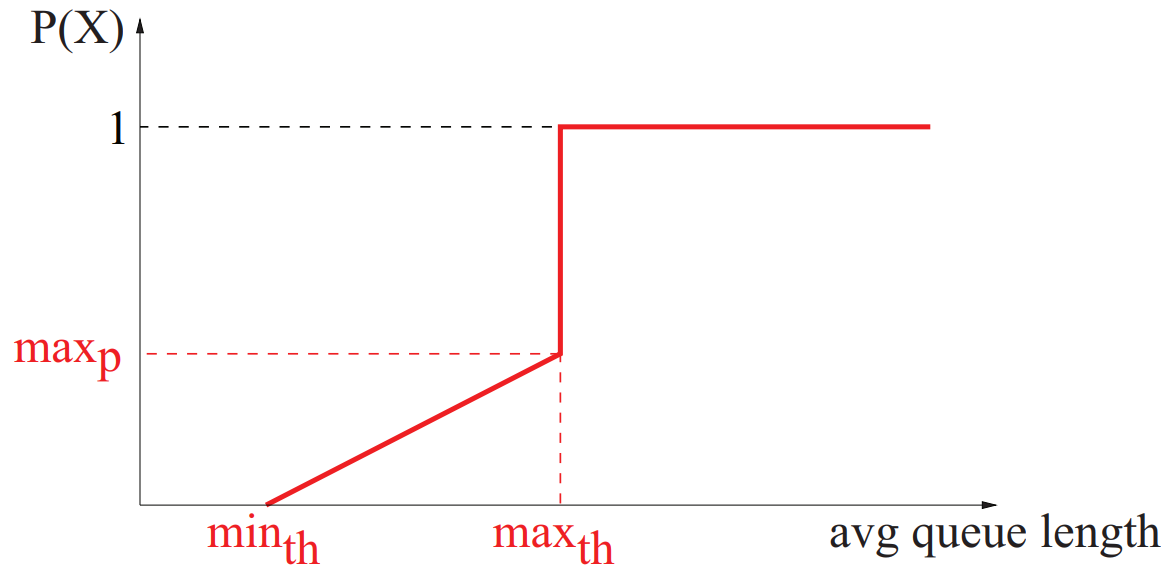
\includegraphics[width=11cm]{2-fundam/REDScheme.PNG}
    \caption{The Random Early Detection (RED) queue management scheme}
    \cite{lochin2011managing}
    \label{fig:redscheme}
\end{figure}

Estudos realizados por \cite{floyd1993random} e \cite{rosolen1999red} mostram que o RED pode melhorar o rendimento e a distribuição dos recursos de rede, enquanto mantém um atraso médio de enfileiramento baixo. No entanto, esse benefício só é alcançado quando o RED está adequadamente configurado sob algumas cargas de tráfego, especificamente quando o comprimento médio da fila não oscila significativamente e permanece abaixo de {$\mathit{max}_\mathit{th}$}.

O artigo publicado por \cite{chung2002analysis} ainda revela que ao utilizar RED combinado com ECN adequadamente configurado, pode resultar em uma taxa de perda de pacotes e atraso de fila muito baixos, o que torna o RED muitas vezes superior ao gerenciamento de fila \emph{drop-tail}, o que também foi confirmado por \cite{silva2017interconnect} ao testar estas configurações em um \emph{cluster} Hadoop.


\subsection{Controlled Delay}

\emph{Controlled Delay} (CoDel) é um algoritmo de escalonamento para o escalonador de rede. Ele é projetado para superar o \emph{bufferbloat} (alta latência em redes com comutação causada pelo excesso de carregamento de pacotes) em \emph{hardware} de rede, como roteadores, definindo limites na experiência de pacotes de rede de atraso à medida que passam pelos \emph{buffers} neste equipamento. Segundo \cite{nichols2012controlling}, CoDel difere dos demais AQMs por:

\begin{itemize}
\item É sem parâmetros - não possui parâmetros para os operadores, usuários ou implementadores ajustarem;
\item Trata as filas de maneiras diferentes mantendo os atrasos baixos enquanto permite picos de tráfego;
\item Controla o atraso e ao mesmo tempo ser insensível a atrasos de ida e volta, taxas de \emph{link} e cargas de tráfego;
\item Se adapta dinamicamente trocando as taxas de \emph{link} sem nenhum impacto negativo na utilização da rede;
\item É simples e eficiente - pode facilmente abranger todo o espectro de baixo custo, pontos de acesso baseados em Linux, roteadores domésticos, e até mesmo roteadores comerciais de silício.
\end{itemize}

O algoritmo do CoDel calcula cada salto de forma independente \cite{nichols2012controlling}. Primeiramente, inicia em um intervalo de 100 milissegundos. O atraso de enfileiramento por pacote é monitorado por meio do salto. À medida que cada pacote é retirado da fila para encaminhamento, o atraso de enfileiramento (quantidade de tempo que o pacote passou esperando na fila) é calculado. O menor atraso de fila para o intervalo é armazenado.

\begin{equation}
Sequencia De Intervalos = (100,\frac{100}{\sqrt2},\frac{100}{\sqrt3},\frac{100}{\sqrt4},\frac{100}{\sqrt5},\frac{100}{\sqrt6},\frac{100}{\sqrt7},...)
\label{eq:CoDel}
\end{equation}

No momento em que o último pacote do intervalo é retirado da fila, se o menor atraso de enfileiramento para o intervalo for maior que 5 milissegundos, esse único pacote é descartado e o intervalo usado para o próximo grupo de pacotes é reduzido. Se o menor atraso de enfileiramento para o intervalo for inferior a 5 milissegundos, o pacote será encaminhado e o intervalo será redefinido para 100 milissegundos. Quando o intervalo é reduzido, isso é feito de acordo com a raiz quadrada inversa do número de intervalos sucessivos nos quais os pacotes foram descartados devido ao atraso excessivo de enfileiramento, conforme demonstrado na expressão 2.1.


\section{Explicit Congestion Notification}

\emph{Explicit Congestion Notification} é uma extensão do protocolo TCP/IP definida em 2001. Com o ECN habilitado a conexão tem alguns aprimoramentos, como por exemplo, realizar notificações de congestionamento de ponta a ponta na rede sem que haja perda de pacotes. Além disso, as fontes podem ser informadas sobre o congestionamento de forma rápida e inequívoca, não havendo necessidade de esperar por um temporizador de retransmissão ou três confirmações duplicadas para inferir um pacote descartado. O ECN pode ser habilitado em qualquer rede LAN/WAN que tenham roteadores ou \emph{switches} nas pontas que ofereçam suporte a esta tecnologia \cite{floyd2000addition}.

\begin{figure}[htp]
    \centering
    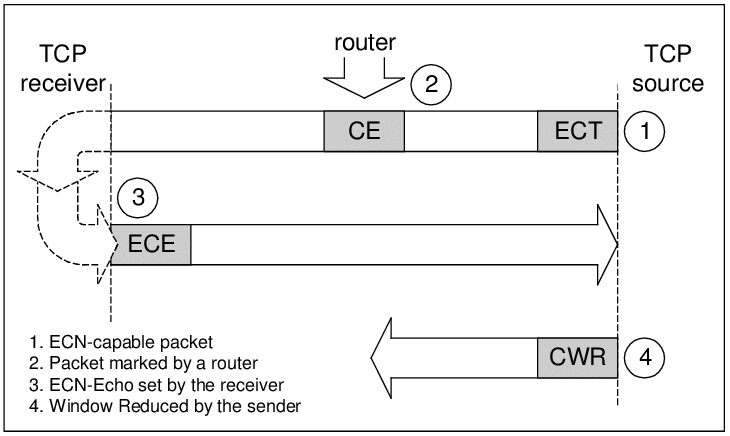
\includegraphics[width=11cm]{2-fundam/Figura_3.jpg}
    \caption{ECN in Action}
    \cite{malowidzki2003simulation}
    \label{fig:ECNinAction}
\end{figure}

O ECN permite roteadores que usam AQMs (por exemplo, RED ou CoDel) marquem os pacotes em caso de congestionamento, em vez de descartá-los. Todo este processo pode ser observado na figura 2.5, em que dois \emph{bits} no cabeçalho IP fornecem quatro marcas possíveis: No-ECN (00), \emph{Congestion Experienced} (CE, 11) e dois pontos de código para \emph{ECN-Capable Transport} (ECT (0), 01; e ECT (1), 10) . Um remetente com capacidade para ECN define ECT (0) ou ECT (1), que pode ser alterado para CE por um roteador para sinalizar o congestionamento. ECN usa dois sinalizadores adicionais no cabeçalho TCP: \emph{ECN-Echo} (ECE) é definido em todos os pacotes do receptor para o remetente para sinalizar a chegada de um pacote com marcação CE até que o remetente defina a janela de \emph{Congestion Window Reduced} (CWR) para reconhecer a ECE. Esses sinalizadores também são usados para negociar o uso de ECN: um iniciador de conexão solicita o ECN configurando ECE e CWR no SYN inicial, e o respondente reconhece configurando ECE no SYN/ACK. Depois de concluir a negociação com êxito, os remetentes podem definir um ponto de código ECT em todos os pacotes subsequentes na conexão \cite{kuhlewind2013state}.

Atualmente o ECN está implementado na maioria dos sistemas operacionais. No entanto, mesmo habilitado por padrão, geralmente está apenas no `modo de servidor': O ECN será negociado se solicitado por um nodo remoto iniciando uma conexão, mas as conexões abertas pelo nodo não tentarão negociar o uso de ECN \cite{kuhlewind2013state}.

\section{MapReduce}

O \emph{MapReduce} surgiu em fevereiro de 2003, quando dois funcionários do Google, Jeffrey Dean e Sanjay Ghemawat buscavam aperfeiçoar o sistema de busca do Google \cite{dean2004mapreduce}. Considerado um modelo de programação altamente avançado para processar grandes conjuntos de dados estruturados e principalmente não estruturados, ele consiste em duas funções:

\begin{itemize}
    \item \emph{Map} (Mapeamento): A função \emph{Map} recebe uma lista ordenada <chave, valor> gerando um conjunto intermediário de dados com o mesmo formato, lista ordenada <chave, valor>.
    \item \emph{Reduce} (Redução): A função \emph{Reduce} é executada para cada chave intermediaria gerada, combinando as chaves associadas.
\end{itemize}


\begin{lstlisting}
map(String key, String value):
	// key: nome do documento
	// value: conteúdo do documento
	for each word w in value:
		EmitIntermediate(w, "1");
reduce(String key, Iterator values):
	// key: uma palavra
	// values: uma lista de contagens
	int result = 0;
	for each v in values:
		result += ParseInt(v);
	Emit(AsString(result)); 
\end{lstlisting}


Durante a execução do \emph{MapReduce}, as funções \emph{Map} e \emph{Reduce} recebem e emitem dados no formato de Listas ordenadas <chave, valor>. Em outras palavras, o algoritmo \emph{Map} é usado para encontrar algo ou resolver pequenos problemas e o \emph{Reduce} para reunir os resultados, gerando assim uma solução para o problema maior. Para ajudar a ilustrar o modelo de programação \emph{MapReduce}, considere o problema de contar quantas vezes cada palavra aparece em um mesmo documento. Pode-se observar acima os pseudocódigos das funções \emph{Map} e \emph{Reduce} de um contador de palavras, em que na fase de mapeamento (\emph{map}) a variável \emph{key} recebe o nome do documento, e a value seu conteúdo, então para cada palavra é emitido no arquivo virtual uma lista <palavra,1>, em seguida, na fase de redução (\emph{reduce}) o \emph{key} recebe novamente uma palavra, enquanto o \emph{iterador values} recebe a todas as listas com a palavra, e então, a variável \emph{result} soma todas, chegando assim na quantidade de vezes em que a palavra aparece no arquivo de entrada.

\begin{figure}[htp]
    \centering
    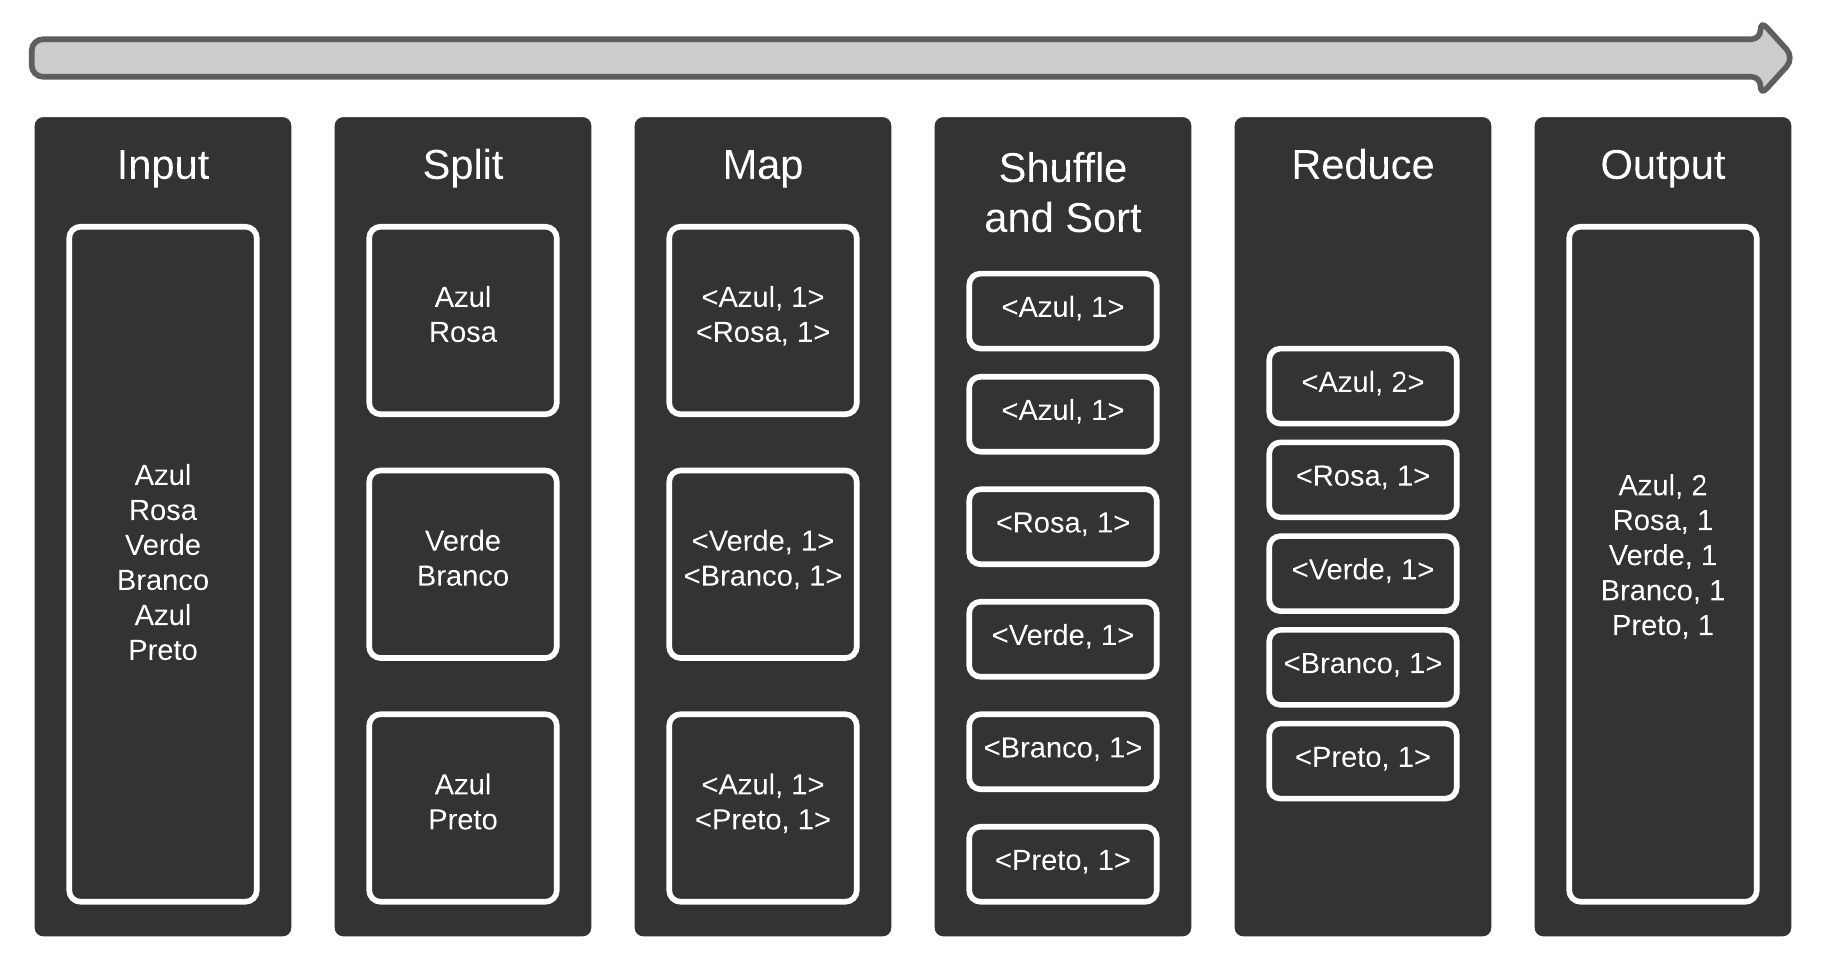
\includegraphics[width=16cm]{2-fundam/Figura_7.jpg}
    \caption{Etapas de uma Aplicação MapReduce WordCount}
    Adaptada de \cite{white2015hadoop}
    \label{fig:Etapas de uma Aplicação MapReduce WordCount}
\end{figure}

Para ilustrar observe a figura 2.6. Ao iniciar uma execução \emph{MapReduce} no \emph{cluster}, o arquivo de entrada é repartido em blocos \emph{(split phase)}, estes blocos são enviados aos nodos do \emph{cluster} responsáveis por realizar um mapeamento dos dados \emph{(map phase)} e emitir várias listas, cada uma contendo uma palavra e uma chave \emph{<word, key>;} nas fases de embaralhamento e ordenação \emph{(shuffle and sort phase)} as listas são ordenadas, e, em seguida, transferidas para a fase de redução \emph{(reduce phase)} que efetua as somas dos valores das chaves e escreve os resultados no arquivo de saída \emph{(output phase)}.

Embora o pseudocódigo do \emph{MapReduce} permaneça o mesmo desde sua criação, a implementação do \emph{Hadoop MapReduce} continua a ser atualizada constantemente \cite{white2009hadoop}; \cite{white2010hadoop}; \cite{white2012hadoop}; \cite{white2015hadoop}.


\section{Apache Hadoop}

Desenvolvido por Doug Cutting e Mike Cafarella e mantido atualmente pela Apache Software Foundation, o ecossistema Hadoop é uma plataforma de código-fonte aberto em Java para armazenamento e processamento de dados em larga escala. A configuração dos \emph{clusters} Hadoop é extremamente fácil, enquanto integridade dos dados, disponibilidade dos nodos, escalabilidade da aplicação e recuperação de falhas são tratadas automaticamente de forma transparente ao usuário, além de possuir um processamento superior as demais tecnologias da área \cite{goldman2012apache}.

A comunidade de \emph{BigData} vem utilizando a Computação de Alto Desempenho (\emph{High-performance Computing} - HPC) e Computação em Grade (\emph{Grid Computing} - GC) por anos para o processamento de dados em larga escala. O problema que surge ao utilizar uma dessas abordagens é de os nodos acessarem a informação através de uma Rede de Área de Armazenamento (\emph{Storage Area Network} - SAN), o que funciona bem para problemas que necessitam de computação extrema, mas, se torna uma fraqueza para aqueles que necessitam acessar grandes volumes de dados constantemente \cite{white2015hadoop}.

Diferentemente do HPC e GC, o Hadoop leva a computação até os dados, ou seja, ele co-localiza os arquivos com os nodos de computação, tornando o acesso mais rápido por ser local \cite{gray2004distributed}. Este recurso do Hadoop é conhecido como `\emph{Data Locality}', sendo o coração do processamento de dados neste Ecossistema e a razão para o seu desempenho superior. Reconhecendo que a largura de banda é o recurso mais precioso em um ambiente de \emph{Data Center} (é fácil saturar os \emph{links} de uma rede com a cópia constante de dados), o Hadoop tenta ao máximo preservar a saúde da mesma modelando explicitamente a topologia da rede \cite{white2015hadoop}.

\subsection{Módulos do Ecossistema Hadoop}

Conforme a documentação do Apache Hadoop \cite{ApacheDocumentation}, a atual versão do ecossistema 3.x é composta por quatro módulos principais, cada um com sua finalidade específica:

\begin{itemize}
    \item \emph{Hadoop Common}: Módulo que contém as bibliotecas e arquivos necessários para o funcionamento total das estruturas do Hadoop.
    \item \emph{Hadoop Distributed File System} (HDFS™): Módulo que age como um sistema de arquivos distribuídos, controlando e armazenando os dados nos nodos, além de permitir largura de banda gigantesca em todo o \emph{cluster}. É altamente tolerante a falhas e pode se recuperar automaticamente.
    \item \emph{Hadoop YARN}: \emph{Framework} que funciona como um \emph{middleware}, gerenciando os recursos disponíveis e fazendo agendamentos dos recursos que serão usados no processamento de dados.
    \item \emph{Hadoop MapReduce}: Contém um sistema baseado em YARN. Quando este módulo está operando, todo o poder computacional do \emph{cluster} é direcionado para as funções \emph{Map} e \emph{Reduce}, permitindo assim o processamento paralelo de grandes conjuntos de dados.
\end{itemize}


\subsection{Processos do Hadoop}

Uma aplicação típica do Hadoop executa cinco processos principais para gerenciar a utilização dos recursos do \emph{Cluster}.

\textbf{\emph{NameNode}:} Na versão 1.x do Hadoop, o \emph{NameNode} era um ponto único de falha (SPOF) em um \emph{cluster HDFS}. Cada \emph{cluster} tinha um único \emph{NameNode} e, se essa máquina ou processo ficasse indisponível, o \emph{cluster} como um todo ficaria indisponível até que o \emph{NameNode} fosse reiniciado ou criado em uma máquina nova. Isso afetava a disponibilidade total do cluster HDFS de duas maneiras principais:

\begin{itemize}

\item No caso de um evento não planejado, como uma falha de nodo, o \emph{cluster} ficava indisponível até que um administrador reiniciasse o \emph{NameNode}.

\item Eventos de manutenção planejada, como atualizações de \emph{software} ou \emph{hardware} na máquina que continha o \emph{NameNode}, resultavam em janelas de tempo de inatividade do \emph{cluster}.

\end{itemize}

O recurso \emph{HDFS High Availability} aborda os problemas acima fornecendo a opção de executar dois (e a partir da versão 3.x mais de dois) \emph{NameNodes} redundantes no mesmo \emph{cluster} em uma configuração ativa/passiva com um \emph{hot standby}. Isso permite um \emph{failover} (método de proteção de sistemas contra falhas, no qual o equipamento de reserva assume automaticamente quando o sistema principal falha) rápido para um novo \emph{NameNode} no caso de falha de uma máquina ou um \emph{failover} iniciado pelo administrador para fins de manutenção e/ou atualização planejada.
    
\textbf{\emph{DataNode}:} Os \emph{DataNodes} são responsáveis por atender as solicitações de leitura e escrita do sistema de arquivos. Os \emph{DataNodes} também executam a criação, exclusão e replicação de blocos mediante instruções do \emph{NameNode}.


\textbf{\emph{ResourceManager}:} O \emph{ResourceManager} (RM) é responsável por rastrear os recursos disponíveis dentro do \emph{cluster} e agendar aplicações (por exemplo, trabalhos \emph{MapReduce}). Antes do Hadoop 2.4, o \emph{ResourceManager} era o único ponto de falha em um \emph{cluster YARN}. O recurso \emph{High Availability} adiciona redundância na forma de um par \emph{Active/Standby ResourceManager}, substituindo assim o RM principal por um secundário caso haja falha.



\textbf{\emph{NodeManager}:} O \emph{NodeManager} é responsável por iniciar e gerenciar contêineres em um nodo. Os contêineres executam tarefas conforme especificado pelo AppMaster. O \emph{NodeManager} executa serviços para determinar a integridade do nodo em que está sendo executado. Os serviços realizam verificações no disco, bem como quaisquer testes especificados pelo usuário. Se qualquer verificação de integridade falhar, o \emph{NodeManager} marcará o nodo como não íntegro e comunicará isso ao \emph{ResourceManager}, que interromperá a atribuição de contêineres ao nodo.


    
\textbf{\emph{SecondaryNameNode}:} O \emph{SecondaryNameNode} mescla o \emph{fsimage} e os arquivos de \emph{log} de edições periodicamente e mantém o tamanho do \emph{log} de edições dentro de um limite. Geralmente é executado em uma máquina diferente do \emph{NameNode} principal, pois seus requisitos de memória são iguais.

O início do processo de \emph{checkpoint} no \emph{NameNode} secundário é controlado por dois parâmetros de configuração:

\begin{itemize}

\item \emph{dfs.namenode.checkpoint.period}, definido como 1 hora por padrão, especifica o atraso máximo entre dois pontos de verificação consecutivos;

\item \emph{dfs.namenode.checkpoint.txns}, definido como 1 milhão por padrão, define o número de transações sem \emph{checkpoint} no \emph{NameNode} que forçarão um \emph{checkpoint} urgente, mesmo que o período do \emph{checkpoint} não tenha sido atingido.

\end{itemize}
O \emph{SecondaryNameNode} armazena o último ponto de verificação em um diretório que é estruturado da mesma forma que o diretório do \emph{NameNode} principal, para que a imagem de verificação esteja sempre pronta para ser lida pelo \emph{NameNode} principal, se necessário.
    


\subsection{Aplicações YARN}

Apache YARN (\emph{Yeat Another Resource Negotiator}) é o sistema de gestão dos recursos dos \emph{clusters} Hadoop, introduzido no ecossistema a partir da versão 2.x para melhorar o desempenho do \emph{MapReduce}, mas também pode ser utilizado em outros paradigmas de computação paralela.

\begin{figure}[htp]
    \centering
    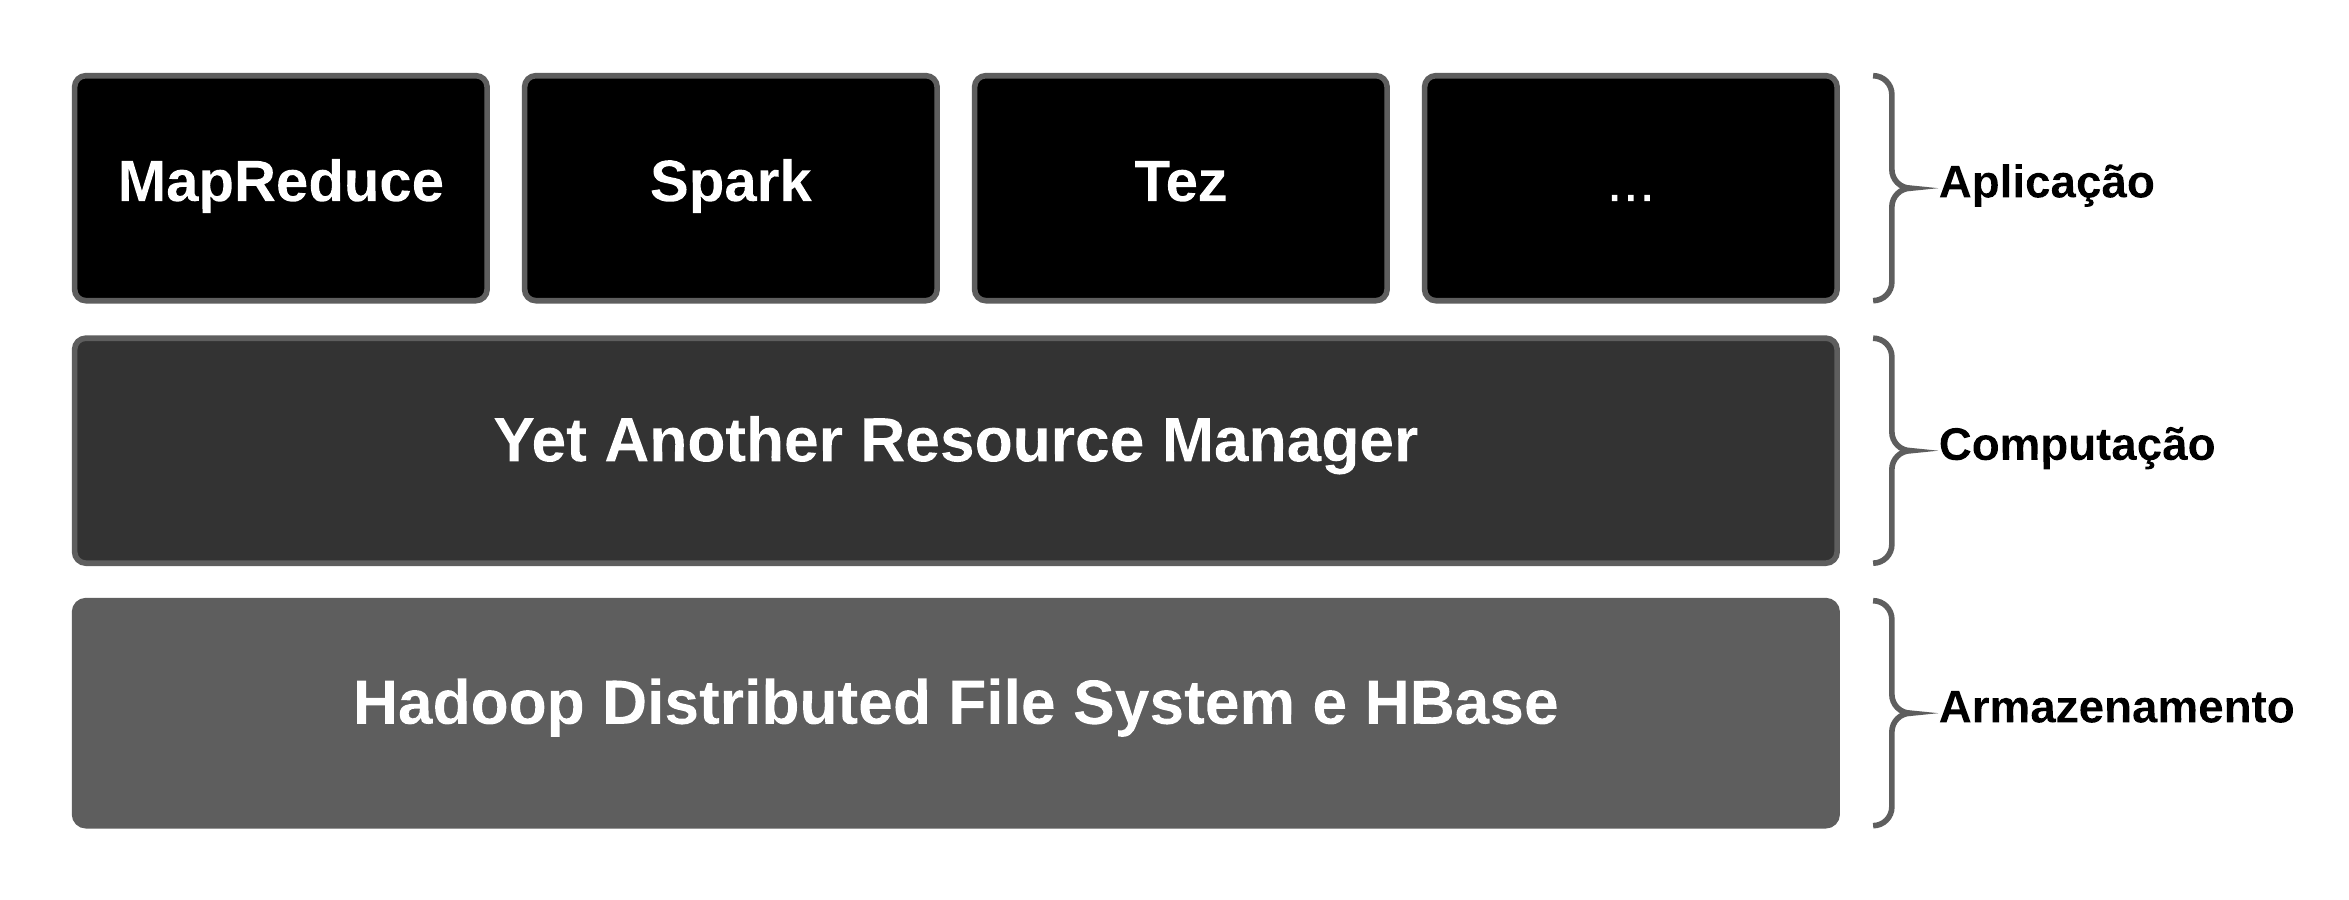
\includegraphics[width=11cm]{2-fundam/Figura_5.jpg}
    \caption{Aplicações YARN}
    Adaptada de \cite{white2015hadoop}
    \label{fig:YARNApplication}
\end{figure}

O YARN fornece APIs para fazer requisições de recursos do \emph{cluster}, mas estas APIs não são utilizadas diretamente no código-fonte das aplicações. Em vez disso, os usuários implementam algoritmos para computação distribuída em linguagem de programação de alto nível a partir de classes abstratas do YARN, que por sua vez, oculta os detalhes de gerenciamento de recursos dos programadores. Na figura 2.7 pode-se observar os \emph{frameworks} de computação distribuída do ecossistema Hadoop como \emph{MapReduce}, Spark, Tez, e assim por diante que são executados como Aplicativos YARN na camada de computação utilizando como sistema de armazenamento o HDFS ou HBase \cite{white2015hadoop}.

Ainda há outra camada de aplicativos acima que podem ser executados nos \emph{frameworks} \emph{MapReduce}, Tez, Spark ou nos três, como por exemplo o Pig, Hive e Crunch, mas não interagem diretamente com o YARN.

O YARN fornece seus principais serviços por meio de dois tipos de \emph{daemon} de longa duração: um \emph{Resource Manager} (um por \emph{cluster}) para gerenciar o uso de recursos no \emph{cluster}, e o \emph{Node Managers} em execução em todos os nós do \emph{cluster} para iniciar e monitorar \emph{Containers}. Um \emph{Container} executa um processo específico da aplicação com um conjunto restrito de recursos (memória, CPU e assim por diante). Dependendo de como o YARN está configurado, um \emph{Container} pode ser um processador Unix ou um cgroup Linux.


\subsection{Hadoop 1.x, 2.x e 3.x}

A seguir apresentamos as principais diferenças entre as versões do Hadoop divididas em dois subsubtópicos para melhor entendimento de novos módulos e as alterações entre os mesmos. Estas inovações impactam diretamente em sua performance e gasto energético, e por isso, foram levadas em conta na definição da metodologia.

\subsubsection{Diferenças entre Hadoop 1.x e 2.x}

Ao longo das atualizações, diversas modificações foram realizadas na estrutura do Ecossistema Hadoop, entre as séries 1.x e 2.x a mais notável é a introdução do YARN entre as camadas do HDFS e \emph{MapReduce}, resultando em uma nova forma (\emph{YARN MapReduce}) de implementar e executar MRJs \cite{white2015hadoop}.

\begin{table}[htbp]
\centering
\caption{A comparison of MapReduce 1 and YARN components}
\label{MR1andYARN}
\begin{tabular}{|l|c|c|} \hline
\textbf{Hadoop 1.x} & \textbf{Hadoop 2.x} \\ \hline
\textbf{MapReduce 1} & \textbf{YARN (MapReduce V2 - NextGen)} \\ \hline
Jobtracker & Resource Manager, Application Master, Timeline Server \\
Tasktracker & Node Manager \\
Slot & Container \\ \hline
\end{tabular}
\end{table}

Na segunda versão do Hadoop, o módulo \emph{Yet Another Resource Negotiator} foi agregado e mudou a arquitetura do arcabouço significativamente como demonstrado na tabela 2.3. O YARN é responsável por gerenciar recursos do \emph{cluster} e agendamento de trabalhos. Nas versões anteriores do Hadoop, essa funcionalidade era integrada ao módulo \emph{MapReduce}, onde era realizada pelo componente \emph{JobTracker}. O \emph{JobTracker} era responsável pelo agendamento, gerenciamento de recursos, monitoramento e reexecução de tarefas com falhas, relatório do status dos trabalhos aos usuários, registro de logs de auditoria, agregação de estatísticas, autenticação de usuários e várias outras funções. A grande quantidade de responsabilidades gerava limitações de escalabilidade. A ideia fundamental do YARN é dividir as duas principais funcionalidades do \emph{JobTracker}, gerenciamento de recursos e agendamento/monitoramento de tarefas para ter um \emph{ResourceManager} global e um \emph{ApplicationMaster} específico de cada aplicação. Ao separar as funções de gerenciamento de recursos do modelo de programação, o YARN delega muitas tarefas relacionadas ao agendamento para componentes por trabalho e se afasta completamente do particionamento estático de recursos para \emph{Mappers} e \emph{Reducers}, considerando os recursos do \emph{cluster} como contínuos, o que traz melhorias significativas para a utilização do mesmo \cite{glushkova2019mapreduce}.

Como analisado por \cite{glushkova2019mapreduce}, para o Hadoop melhorar o desempenho geral, bem como a utilidade e compatibilidade com outros aplicativos de processamento de dados distribuídos, alguns requisitos foram adicionados, como alta utilização dos recursos do \emph{cluster}, alto nível de confiabilidade e disponibilidade, suporte para diversidade de modelos de programação e modelos de recursos flexíveis. Assim, a arquitetura da segunda versão do Hadoop passou por melhorias significativas, introduzindo o YARN, um módulo de gerenciamento de recursos separado que altera visivelmente a arquitetura geral, em que desacopla o modelo de programação da infraestrutura de gerenciamento de recursos e delega muitas funções de agendamento para os componentes da aplicação. Os recursos do \emph{cluster} agora estão sendo considerados contínuos, portanto, não há particionamento estático de recursos (ou seja, uma divisão entre \emph{slots} de \emph{mappers} e \emph{reducers}). Então, as tarefas de mapeamento e redução competem agora pelos mesmos recursos. Estas diferenças causam em média de 11\% a 13.5\% de redução no custo de MRJs entre as versões 1.x e 2.x do Hadoop.

\subsubsection{Diferenças entre Hadoop 2.x e 3.x}

O Apache Hadoop 3.x incorpora uma série de melhorias significativas em relação à sua linha de lançamentos anteriores Hadoop 2.x. Uma das principais modificações é o \emph{Erasure Coding} (EC), um método para armazenar dados de forma duradoura com economia de espaço significativa em comparação a forma antiga (replicação). O EC fornece o mesmo nível de tolerância a falhas com um menor espaço de armazenamento consumido, em suas configurações típicas a sobrecarga de armazenamento não é superior a 50\%. A integração do EC ao HDFS pode melhorar a eficiência do armazenamento, ao mesmo tempo em que oferece durabilidade de dados semelhante às implantações HDFS tradicionais baseadas em replicação. Por exemplo, um arquivo replicado na versão 2.x do Hadoop com 6 blocos consumiria (6x3=18) 18 blocos de espaço em disco, mas, na versão 3.x com a implantação EC (6 de dados, 3 de paridade), ele consumirá apenas 9 blocos de espaço em disco \cite{hadoop3.0.0release}.


%Passando para português

\begin{table}[htbp]
\centering
\caption{Comparação entre Hadoop 2.x e Hadoop 3.x}
\label{Hadoop2andHadoop3}
\begin{tabular}{|l|c|c|} \hline
\textbf{Atributos} & \textbf{Hadoop 2.x} & \textbf{Hadoop 3.x} \\ \hline
Lida com Falhas & Através da Replicação & Através do \emph{Erasure Coding}\\\hline
Sobrecarga de Armazenamento & 200\% no HDFS & 50\% no HDFS\\\hline
Sistema de Arquivos & DFS, FTP e Amazon S3 & Anteriores + MADLFS\\\hline
Intervenção Manual & Não é necessária & Não é necessária\\\hline
Escalabilidade & Limitado a 10,000 nodos & Mais de 10,000 nodos\\\hline
Gerenciamento de Recursos & YARN & YARN\\\hline
Balanceamento dos Dados & Usa balanceador HDFS & Usa balanceador Intra-dados\\
\hline
\end{tabular}
\end{table}



Como pode-se observar na tabela 2.4 as principais mudanças são a implementação do \emph{Erasure Coding} que reduz a sobrecarga de armazenamento em 150\% em relação a replicação, aumento da escalabilidade para mais de 10.000 nodos e o balanceamento de dados que agora é feito de forma interna pelos nodos.

Estudos comparativos realizados por \cite{masur2017preliminary} mostram que o Hadoop 3.x leva vantagem em média de 40\% em operações \emph{TeraSort} sobre a versão anterior, e esta porcentagem tende a aumentar para mais de 50\% quando envolve operações de leitura e escrita, o que resulta em MRJs mais rápidos na versão atual. Os resultados destas pesquisas podem ser observados na tabela 2.5.

\begin{table}[htbp]
\centering
\caption{Tempo de execução das tarefas no Hadoop 2.x e 3.x}
\label{Hadoop2andHadoop3Comparison}
\begin{tabular}{|l|c|c|} \hline
\textbf{Operação} & \textbf{Hadoop 2.x} & \textbf{Hadoop 3.x} \\ \hline
Escrita 500 MB & 65 Segundos & 27 Segundos\\\hline
Escrita 1 GB & 103 Segundos & 27 Segundos\\\hline
Escrita 10 GB & 214 Segundos & 118 Segundos\\\hline
Leitura 500 MB & 62 Segundos & 19 Segundos\\\hline
Leitura 1 GB & 125 Segundos & 16 Segundos\\\hline
Leitura 10 GB & 148 Segundos & 48 Segundos\\\hline
TeraSort 1 GB & 176 Segundos & 83 Segundos\\\hline
TeraSort 10 GB & 423 Segundos & 275 Segundos\\
\hline
\end{tabular}
\end{table}

Neste estudo feito por \cite{masur2017preliminary}, o \emph{benchmark MRBench} de \cite{noll2011benchmarking} foi utilizado para testar a camada \emph{MapReduce} de ambas as versões do Hadoop, e o \emph{AverageTime} levado para completar duas tarefas de mapeamento e uma de redução foi contabilizado para cada uma delas. Várias operações de escrita, leitura e classificação foram realizadas em ambas as versões do Hadoop para comparação; e os resultados indicam que o desempenho do Hadoop 3.x excede o do Hadoop 2.x por uma grande margem, especialmente com relação ao tempo médio gasto para a conclusão das tarefas de Mapeamento (\emph{Mappers}) e Redução (\emph{Reducers}).

\subsection{YARN Scheduler Load Simulator}

O Agendador de tarefas do YARN é uma área fértil em interesses com diferentes implementações, por exemplo, agendamentos \emph{First In First Out}, \emph{Capacity} e \emph{Fair}, ao mesmo tempo em que várias otimizações também são feitas para melhorar o desempenho dos agendadores para diferentes cenários e cargas de trabalhos. Cada algoritmo do agendador tem seu próprio conjunto de recursos e orienta as decisões de agendamento por muitos fatores, como equidade, garantia de capacidade, disponibilidade de recursos, entre outras. É muito importante avaliar um algoritmo do agendador antes de implantá-lo em um \emph{cluster} de produção. Infelizmente, atualmente não é trivial avaliar um algoritmo do escalonador, pois, avaliar em um \emph{cluster} real é sempre demorado e custoso, além de ser muito difícil encontrar um \emph{cluster} grande o suficiente. Consequentemente, seria bastante útil um simulador que possa prever quão bem será um algoritmo de agendamento para alguma carga de trabalho específica.

\begin{figure}[htbp]
    \centering
    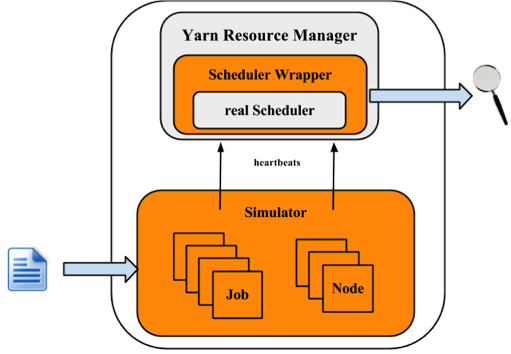
\includegraphics[width=10.2cm]{2-fundam/Figura_9.jpg}
    \caption{Arquitetura do SLS}
    \cite{ApacheSLS}
    \label{fig:ApacheSLS}
\end{figure}

\begin{figure}[htbp]
    \centering
    \label{fig:SLSPanel_1}
    
    \subfloat[SLS - Cluster Memory \label{fig:SLSPanel_2}]{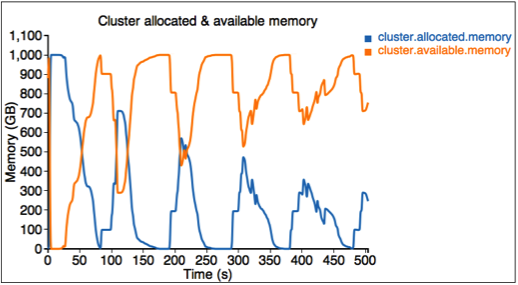
\includegraphics[width=8cm]{2-fundam/SLS - Cluster Memory.png}}\hfill
    \subfloat[SLS - Queue Allocated Memory
    \label{fig:SLSPanel_3}]{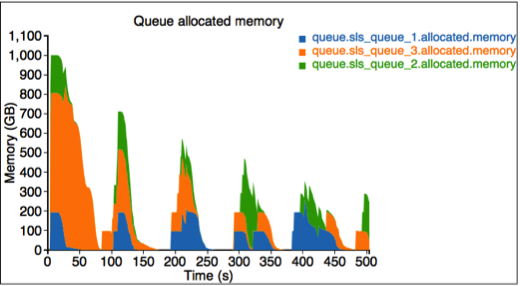
\includegraphics[width=8cm]{2-fundam/SLS - Queue Allocated Memory.png}}
    
    \subfloat[SLS - Running Apps Containers \label{fig:SLSPanel_4}]{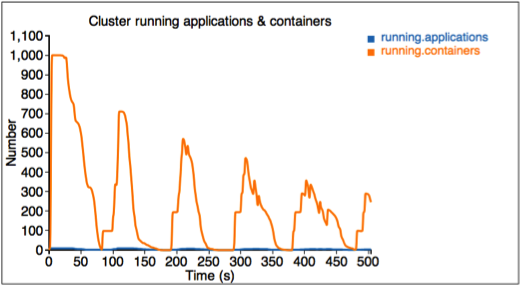
\includegraphics[width=8cm]{2-fundam/SLS - Running Apps Containers.png}}\hfill
    \subfloat[SLS - Scheduler Operation Timecost
    \label{fig:SLSPanel_5}]{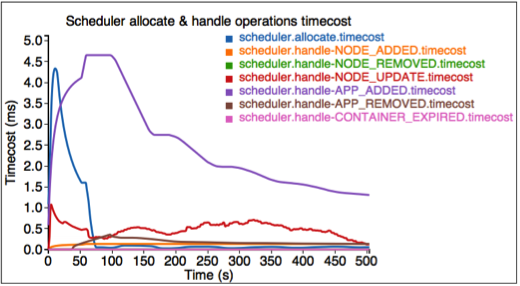
\includegraphics[width=8cm]{2-fundam/SLS - Scheduler Operation Timecost.png}}    
    
    \subfloat[SLS - Track Queue
    \label{fig:SLSPanel_6}]{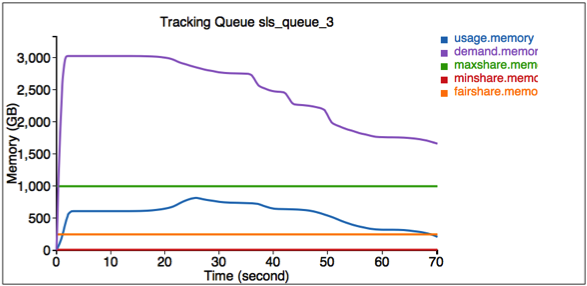
\includegraphics[width=8cm]{2-fundam/SLS - Track Queue.png}}\hfill
    \subfloat[SLS - Track Job
    \label{fig:SLSPanel_7}]{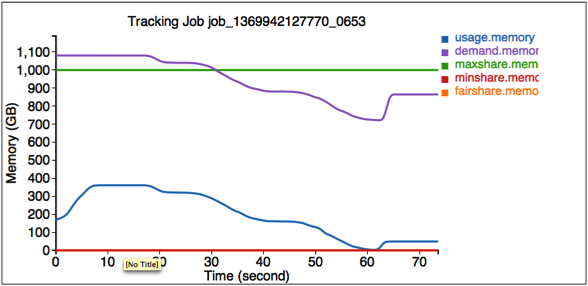
\includegraphics[width=8cm]{2-fundam/SLS - Track Job.png}}       
    
    \caption{Gráficos gerados em tempo real pelo YARN Scheduler Load Simulator}
    \cite{ApacheSLS}
\end{figure}

O \emph{YARN Scheduler Load Simulator} (SLS) é uma ferramenta que pode simular \emph{clusters} YARN em grande escala e cargas de aplicativos em uma única máquina. Este simulador é uma ferramenta para pesquisadores e desenvolvedores criarem protótipos de novos recursos de agendamento e prever seu comportamento e desempenho com uma quantidade razoável de confiança, ajudando assim a inovação. O simulador exercitará o \emph{YARN ResourceManager} real removendo o fator de rede, simulando \emph{NodeManagers} e \emph{ApplicationMasters} por meio do tratamento e envio de eventos de pulsação NM/AMs de dentro da mesma JVM. Para manter o controle do comportamento e desempenho do planejador, um embrulhador do agendador envolverá o agendamento real \cite{ApacheSLS}.



Como pode-se observar na figura 2.8, o SLS obtém dados de rastreios de cargas de trabalhos ou distribuições de carga sintética e gera as informações de \emph{cluster} e aplicações. Para cada NM e AM, o simulador constrói uma instância de simulador para simular sua execução. Todos os simuladores NM/AM são executados em um \emph{Pool of Threads}. O simulador reutiliza o \emph{YARN Resource Manager} e cria um \emph{Wrapper} a partir do agendador. O \emph{Scheduler Wrapper} pode rastrear os comportamentos do planejador e gerar vários \emph{logs}, que são as saídas do simulador e podem ser analisados posteriormente.

Ao observar a figura 2.9 é possível notar que o SLS produz diversas métricas em tempo real durante a execução, incluindo:

\begin{itemize}
    \item Usos de recursos para todo o \emph{cluster} e cada fila, que podem ser utilizados para configurar o \emph{cluster} e a capacidade da fila;
    \item O rastreamento detalhado da execução do aplicativo (registrado em relação ao tempo simulado), que pode ser analisado para entender e validar o comportamento do planejador (tempo de giro de tarefas individuais, rendimento, \emph{fairness}, garantia de capacidade, etc.);
    \item Várias métricas importantes do algoritmo do planejador de tarefas, como custo de tempo de cada operação do planejador (alocar, manipular, etc.), que podem ser utilizadas pelos desenvolvedores do Hadoop para encontrar os pontos de código e os limites de escalabilidade.
\end{itemize}

\section{Considerações Finais}

Neste capítulo foram descritos os conceitos explorados nesta dissertação. Primeiramente,
na seção 2.1 foi abordada a definição do \emph{Energy Efficient Ethernet} e seus dois modos de configuração \emph{Fast Wake Mode} e \emph{Deep Sleep Mode} os quais possuem um diferente consumo de energia, 60\% e 10\% respectivamente. Já na seção 2.2, foi descrito o \emph{Packet Coalescing}, um agrupamento de pacotes como forma de limitar o número de interrupções de recebimento de pacotes e, como resultado, diminuir a quantidade de processamento necessária. Isso pode aumentar a latência da rede, mas em contrapartida, aumenta as chances de que a rede consuma uma quantidade menor de energia, principalmente quando aliada ao EEE.

A seção 2.3 descreve o \emph{Active Queue Management}, uma política implementada em roteadores e comutadores para descartar pacotes dentro de um \emph{buffer} associado a um \emph{Network Interface Controller} (NIC) antes que o \emph{buffer} fique cheio, geralmente com o objetivo de reduzir o congestionamento da rede ou melhorar a latência de ponta a ponta.  Em seguida, foram descritos dois tipos de AQM, o \emph{Random Early Detection} (RED) que descarta pacotes preventivamente antes que o \emph{buffer} fique completamente cheio; e o \emph{Controlled Delay} (CoDel) que defini limites no atraso dos pacotes à medida que passam pelos \emph{buffers} no equipamento. A seção 2.4 aborda o \emph{Explicit Congestion Notification}, uma extensão do protocolo TCP/IP que pode ser utilizada juntamente ao RED e CoDel. Com o ECN habilitado a conexão tem alguns aprimoramentos, como por exemplo, realizar notificações de congestionamento de ponta a ponta na rede sem que haja a perda de pacotes.

No item 2.5 é descrito o \emph{MapReduce}, um modelo de programação avançado para processar grandes conjuntos de dados estruturados e principalmente não estruturados que consiste em duas funções, \emph{Map} (usado para encontrar algo ou resolver pequenos problemas) e \emph{Reduce} (usado para reunir os resultados, gerando assim uma solução para o problema maior).

Por fim, a seção 2.6 abrange os conceitos do Apache Hadoop (uma plataforma de código-fonte aberto para armazenamento e processamento de dados em larga escala), como seus principais módulos que compõem o ecossistema central; processos executados na JVM durante uma aplicação; o YARN - sistema de gestão dos recursos dos \emph{Clusters Hadoop}; as diferenças entre as versões 1.x, 2.x e 3.x do Hadoop; além do \emph{YARN Scheduler Load Simulator} (SLS), uma ferramenta que pode simular \emph{clusters YARN} em grande escala e cargas de aplicativos em uma única máquina.

%=====================================================
